\documentclass[11pt]{article}

\usepackage{amsmath}
\usepackage{amssymb}
\usepackage[margin=0.68in]{geometry}
\usepackage{booktabs}
\usepackage{enumitem}
\usepackage{fancyhdr}
\usepackage{graphicx}
\usepackage[table]{xcolor}
\usepackage[hidelinks]{hyperref}
\usepackage{listings}
\usepackage{microtype}
\usepackage{tabularx}
\usepackage{titlesec}
\graphicspath{{docs/lessons/assets/}{../assets/}}

\definecolor{Ink}{gray}{0}
\definecolor{CodeGray}{gray}{0.96}
\hypersetup{
  pdftitle={ADK Lesson 033: Calibration Console},
  pdfauthor={Kevin Shanahan},
  pdfsubject={Deterministic joystick selection, encoder trim, atomic commit, cancel, and circuit-native evidence},
  pdflang={en-US}
}
\pagestyle{fancy}
\fancyhf{}
\lhead{\textsc{ADK Lesson 033}}
\rhead{Calibration Console}
\cfoot{\thepage}
\setlength{\headheight}{14pt}
\setlength{\parindent}{0pt}
\setlength{\parskip}{5pt}
\setlist{nosep,leftmargin=1.45em}
\titleformat{\section}{\Large\bfseries\color{Ink}}{\thesection}{0.5em}{}
\titleformat{\subsection}{\large\bfseries\color{Ink}}{\thesubsection}{0.5em}{}
\lstdefinestyle{adkcpp}{
  language=C++,
  backgroundcolor=\color{CodeGray},
  basicstyle=\ttfamily\small,
  keywordstyle=\color{Ink}\bfseries,
  commentstyle=\color{Ink},
  columns=fullflexible,
  keepspaces=true,
  showstringspaces=false,
  frame=single,
  rulecolor=\color{Ink},
  breaklines=true,
  tabsize=4
}
\newcommand{\checkbox}{\(\square\)}
\newcommand{\blank}[1]{\rule{#1}{0.4pt}}
\newcommand{\lessonbox}[1]{%
  \begin{center}\fcolorbox{Ink}{white}{\parbox{0.92\linewidth}{#1}}\end{center}}

\begin{document}

\begin{center}
  {\Huge\bfseries Calibration Console}\\[4pt]
  {\Large Select, preview, trim, commit, or cancel}\\[8pt]
  \textit{A deterministic value editor with no storage or actuator path}
\end{center}

\begin{tabularx}{\linewidth}{@{}>{\bfseries}l X >{\bfseries}l X@{}}
Lesson & 033 --- project & Time & 180--240 minutes\\
Prerequisites & Lessons 031 and 032 & Board & Arduino Mega 2560\\
Evidence & TP-X, TP-Y, TP-A, TP-B, LCD, RGB, four LEDs &
Status & active integration; bench open\\
Energy class & E1: USB, passive controls, resistor-limited indicators\\
\end{tabularx}

\lessonbox{\textbf{Boundary.} This project edits two bounded calibration
values in volatile memory. It writes no EEPROM and controls no motor, servo,
relay, heater, lock, or other actuator. Calibration output is presentation
only. Remove USB power to stop physical work; software shutdown is lifecycle
behavior, not an emergency stop.}

\section{Mission and learning outcomes}

\[
\text{raw controls}\rightarrow\text{interpreted events}\rightarrow
\text{bounded preview}\rightarrow\text{explicit commit or cancel}.
\]

Lesson 031 supplies raw and interpreted joystick evidence. Lesson 032 supplies
valid Gray-code edges, invalid-transition evidence, and a separate encoder
button. Lesson 033 coordinates their values in one hardware-neutral console.

After the lesson, you can:
\begin{itemize}
  \item distinguish a committed pair from a transient preview;
  \item explain why selection dead bands preserve prior intent;
  \item apply coarse joystick motion before one-unit encoder trim;
  \item prove atomic commit and exact cancel rollback with deterministic replay;
  \item separate raw test-point, component, project, and presentation evidence;
  \item record acquisition, inactive state, and resource release separately.
\end{itemize}

\section{Monochrome orientation drawing}

\begin{center}
% ADK visual: pencil
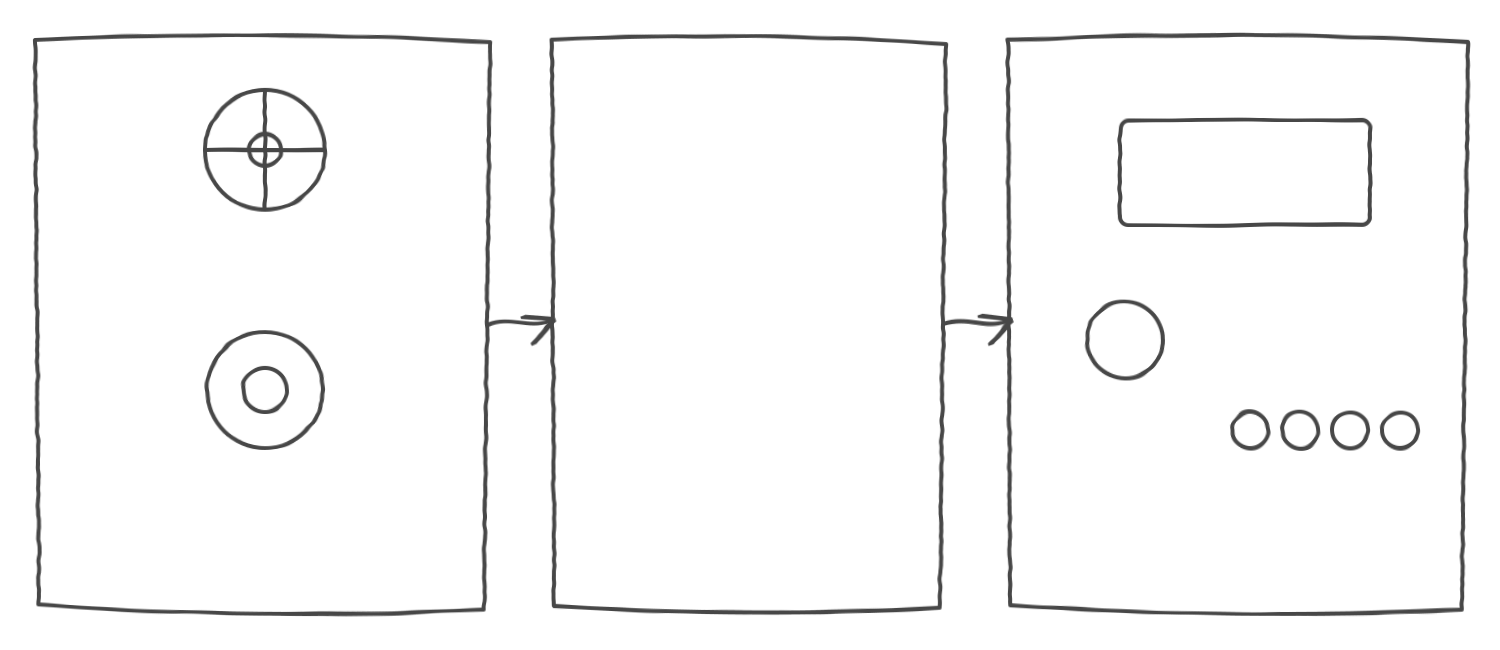
\includegraphics[width=0.96\linewidth]{033-console-orientation-pencil.png}

\begin{tabularx}{0.96\linewidth}{@{}>{\centering\arraybackslash}X
  >{\centering\arraybackslash}X >{\centering\arraybackslash}X@{}}
\textbf{Joystick + Encoder} & \textbf{Mega 2560 + console} &
\textbf{Presentation}\\
TP-X: field & supplied-time update & LCD: field/values\\
TP-Y: coarse preview & commit/cancel policy & RGB: console state\\
TP-A + TP-B: trim & & four LEDs: preview nibble\\
button: cancel & & optional piezo: acknowledgement
\end{tabularx}

\small\textit{Alternative text: a left-to-right orientation diagram. The
joystick provides field selection at TP-X and coarse preview at TP-Y. The
encoder provides trim phases at TP-A and TP-B plus a cancel button. A
supplied-time console presents field and values on an LCD, state on an RGB
LED, and the selected preview's high nibble on four separate LEDs.}
\end{center}

This drawing expresses evidence flow, not an exact revision pinout. The
qualified Lesson 031 and 032 specimen records and canonical sketch supply the
authoritative pin table. Never infer a KY-series marking, pin order, voltage,
or pull policy from the retail kit name or this orientation drawing.

\begin{tabularx}{\linewidth}{@{}l l X@{}}
\toprule
Role & Mega pins & Canonical connection\\
\midrule
joystick X / TP-X & A0 & inspected module X output\\
joystick Y / TP-Y & A1 & inspected module Y output\\
joystick Select & D22 & inspected module switch output\\
encoder A / TP-A & D24 & inspected module A/CLK output\\
encoder B / TP-B & D25 & inspected module B/DT output\\
encoder Cancel & D26 & inspected module switch output\\
preview nibble & D27--D30 & each pin to 1 k\(\Omega\), LED anode; cathode to GND\\
16x2 LCD & D31--D36 & RS, EN, D4, D5, D6, D7\\
common-cathode RGB & D5--D7 & one 330 \(\Omega\) resistor per channel\\
\bottomrule
\end{tabularx}

The exact inspected-module record determines supply, ground, and signal pin
order. This table does not authorize an unidentified lookalike.

\begin{tabularx}{\linewidth}{@{}l X X@{}}
\toprule
Point & Observe relative to Mega GND & Interpret only after comparison with\\
\midrule
TP-X & horizontal wiper, inside board rails & joystick raw X and selected field\\
TP-Y & vertical wiper, inside board rails & joystick raw Y and coarse preview\\
TP-A & encoder A/CLK logic level & ordered A/B phase and encoder snapshot\\
TP-B & encoder B/DT logic level & ordered A/B phase and encoder snapshot\\
\bottomrule
\end{tabularx}

\section{State and value contract}

\begin{tabularx}{\linewidth}{@{}l X X@{}}
\toprule
State & Narrow meaning & Circuit-native presentation\\
\midrule
Selecting & choose Minimum or Maximum & blue RGB\\
Editing & change only the selected preview field & amber RGB\\
Committed & atomic-commit acknowledgement & green RGB\\
Cancelled & exact-rollback acknowledgement & violet RGB\\
Fault & invalid input, time, configuration, or invariant & red RGB\\
\bottomrule
\end{tabularx}

The engine owns no endpoint and performs no I/O. The caller supplies time and
one input value, then reads a stable snapshot. Its public values are a
\texttt{TimePoint}, a console input, and a console snapshot; the latter two
are named \texttt{CalibrationConsoleInput} and
\texttt{CalibrationConsoleSnapshot}. Construction is inert.

In Selecting, X below \(-500\) chooses Minimum and X above \(500\) chooses
Maximum. The center band preserves the current field. Select copies both
committed values to preview and enters Editing.

In Editing, Y outside \(-500\ldots500\) maps to a coarse candidate across the
configured range. Centered Y holds the candidate. Encoder delta is then a
one-unit trim. At all times:
\[
\begin{aligned}
\mathrm{lowerLimit} &\leq \mathrm{minimum}
 \leq \mathrm{maximum}-\mathrm{minimumSeparation},\\
\mathrm{minimum}+\mathrm{minimumSeparation}
 &\leq \mathrm{maximum}\leq \mathrm{upperLimit}.
\end{aligned}
\]

Select commits both values atomically. Cancel wins over simultaneous Select,
restores both preview values, and commits nothing. Acknowledgement lasts the
configured duration before returning to Selecting.

\lessonbox{\textbf{Fault rule.} Invalid input, backward non-wrapping time, or
an impossible configuration enters Fault and commits no value. Recovery
requires explicit shutdown and reinitialization. Shutdown clears transient
events but leaves the last committed pair inspectable.}

\section{Narrative Mega adapter}

The adapter observes the two components, decides through the value-only
console, then presents one snapshot. Presentation cannot call back into the
engine.

\begin{lstlisting}[style=adkcpp]
void loop ()
{
    const adk::TimePoint now (millis ());

    observeControls (now);
    decideCalibration (now);
    presentPreview ();
}
\end{lstlisting}

Setup reads as acquire inputs, acquire indicators, initialize console, show
ready. The LCD presents the selected field plus committed and preview values.
Four separately resistor-limited LEDs present the high nibble of the selected
preview, preserving a non-Serial result if the LCD adapter fails. RGB presents
state. A short piezo acknowledgement is optional supporting evidence.

\section{Preview, trim, commit, and cancel experiment}

\begin{enumerate}
  \item With USB removed, record the exact joystick and encoder revisions.
        Compare every marking and pin label with their qualified records.
  \item Inspect supply and ground, TP-X, TP-Y, TP-A, TP-B, each LED resistor,
        RGB polarity, and common ground before applying power.
  \item Predict Minimum remains selected with centered X. Start the fixture,
        observe blue, and reconcile TP-X with raw X and the LCD field.
  \item Move X past the positive threshold. Predict Maximum, then return X to
        center and verify that the selection remains stable.
  \item Press joystick Select. Predict amber and
        preview \(=\) committed. Move Y beyond its threshold; observe a coarse
        change on the LCD and four-LED nibble.
  \item Turn through one valid encoder edge sequence. Predict one unit of trim.
        Reconcile TP-A/TP-B order, encoder delta, preview, and presentation.
  \item Press Select. Predict one atomic commit and green acknowledgement.
  \item Begin another edit and press the encoder button. Predict violet,
        nothing committed, and exact restoration of both preview values.
  \item Present Select and Cancel together. Predict Cancel precedence.
  \item Invoke shutdown separately, record inactive presentation, check
        resource release with the named method, and then remove USB.
\end{enumerate}

\begin{tabularx}{\linewidth}{@{}X X X@{}}
\toprule
Step & Prediction & Observation and interpretation\\
\midrule
field threshold and center hold & \blank{1.35in} & \blank{1.9in}\\
coarse Y endpoint & \blank{1.35in} & \blank{1.9in}\\
one encoder trim & \blank{1.35in} & \blank{1.9in}\\
atomic commit & \blank{1.35in} & \blank{1.9in}\\
cancel rollback & \blank{1.35in} & \blank{1.9in}\\
simultaneous cancel/select & \blank{1.35in} & \blank{1.9in}\\
\bottomrule
\end{tabularx}

\section{Evidence chain and diagnosis}

\begin{center}
% ADK visual: pencil
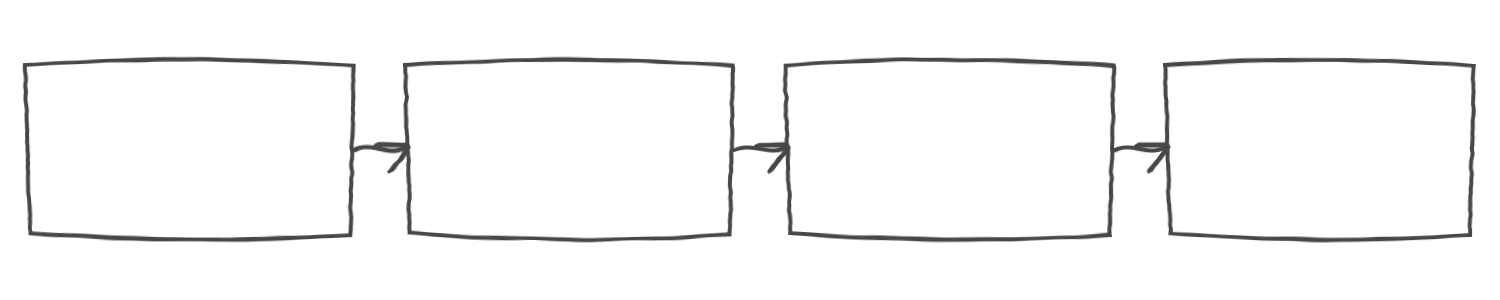
\includegraphics[width=0.96\linewidth]{033-evidence-chain-pencil.png}

\small\textbf{TP-X / TP-Y / TP-A / TP-B}
\(\rightarrow\) \textbf{component snapshots}
\(\rightarrow\) \textbf{console snapshot}
\(\rightarrow\) \textbf{LCD / RGB / four LEDs}

\small\textit{Alternative text: pencil evidence chain from TP-X, TP-Y, TP-A,
and TP-B through component snapshots and the console snapshot to the LCD,
RGB LED, and four indicator LEDs.}
\end{center}

Agreement at one link does not prove the next. An LCD value does not prove the
raw voltage; a valid phase sequence does not prove a commit; a dark LED does
not prove pin release. Serial output may label an observation, but it is never
the only evidence route.

\begin{tabularx}{\linewidth}{@{}X X@{}}
\toprule
Observation & Stop, inspect, and interpret\\
\midrule
field changes while X is centered & compare TP-X, calibration, and thresholds\\
preview jumps by more than expected & separate Y coarse mapping from encoder trim\\
encoder count changes on invalid jump & inspect TP-A/TP-B order and invalid counter\\
only one value restores on Cancel & reject the adapter or engine evidence\\
red state appears & record status; reinitialize only after correcting cause\\
LED nibble disagrees with LCD & inspect snapshot-to-presentation mapping\\
out-of-rail test point or hot part & remove USB and troubleshoot unpowered\\
\bottomrule
\end{tabularx}

\section{Deterministic replay worksheet}

Host tests supply every timestamp and input. They cover every state and
transition, both fields, center stability, coarse endpoints, every clamp,
encoder trim, atomic commit, rollback, simultaneous events, invalid ranges,
input failure, acknowledgement boundaries, rollover, restart, and shutdown.

\begin{lstlisting}[style=adkcpp]
make calibration-console-test
make host-test-exceptions
make arduino-Lesson033CalibrationConsole
make size-check
\end{lstlisting}

\begin{tabularx}{\linewidth}{@{}l X X X@{}}
\toprule
Frame & Predicted state/value & Replay result & Reconciliation\\
\midrule
centered Selecting & \blank{1.0in} & \blank{1.0in} & \blank{1.0in}\\
coarse Maximum edit & \blank{1.0in} & \blank{1.0in} & \blank{1.0in}\\
one negative trim & \blank{1.0in} & \blank{1.0in} & \blank{1.0in}\\
Select + Cancel & \blank{1.0in} & \blank{1.0in} & \blank{1.0in}\\
invalid input & \blank{1.0in} & \blank{1.0in} & \blank{1.0in}\\
\bottomrule
\end{tabularx}

Run the same recording twice. First final snapshot bytes:
\blank{1.4in}; second: \blank{1.4in}. Explain any difference:
\blank{2.0in}.

\section{Claim--evidence--reasoning}

\begin{tabularx}{\linewidth}{@{}X X X@{}}
\toprule
Claim & Evidence to record & What it cannot prove\\
\midrule
field selection is correct & TP-X, raw X, field snapshot & endpoint release\\
trim is one unit & TP-A/B sequence, delta, preview & electrical identity\\
commit is atomic & before/after pair and state & persistent storage\\
cancel restores values & committed and preview pair & actuator safety\\
shutdown is inactive & presentation and pin level & USB power removal\\
\bottomrule
\end{tabularx}

Chosen claim: \blank{2.0in}\\[7pt]
Evidence: \blank{5.7in}\\[7pt]
Reasoning and limits: \blank{4.9in}

\section{Open hardware acceptance record}

\textbf{Software gates are not a physical result.} Keep this card open until
the exact board, specimens, supply, instruments, measurements, date, and
reviewer are present.

\begin{tabularx}{\linewidth}{@{}l X l X@{}}
\toprule
Mega/revision & \blank{1.25in} & Commit & \blank{1.15in}\\
Joystick/encoder & \blank{1.25in} & Markings & \blank{1.15in}\\
Supply/instrument & \blank{1.25in} & Tool versions & \blank{1.15in}\\
Operator/date & \blank{1.25in} & Reviewer & \blank{1.15in}\\
\bottomrule
\end{tabularx}

\begin{itemize}
  \item[\checkbox] unpowered identity, pinout, polarity, resistors, and common
        ground inspected against qualified records;
  \item[\checkbox] acquisition and rollback observed separately from safe state;
  \item[\checkbox] TP-X/TP-Y raw axes and TP-A/TP-B phase evidence recorded;
  \item[\checkbox] both fields, coarse mapping, trim, clamps, commit, cancel,
        simultaneous-event precedence, and fault presentation reconciled;
  \item[\checkbox] repeated replay produced identical snapshots;
  \item[\checkbox] shutdown inactive state and resource release recorded as
        separate claims;
  \item[\checkbox] USB power-removal result recorded.
\end{itemize}

Prediction: \blank{5.8in}\\[8pt]
Observation: \blank{5.7in}\\[8pt]
Interpretation and limits: \blank{4.9in}

\lessonbox{\textbf{Stop rule.} Remove USB power for a hot part, unstable
supply, wrong polarity, missing resistor, out-of-rail TP-X/TP-Y/TP-A/TP-B,
unexpected output, or disagreement between the qualified pin table and
breadboard. Never discover an unknown module rating by experiment.}

\section{Reproduce and reference}

\begin{lstlisting}[style=adkcpp]
make calibration-console-test
make host-test-exceptions
make host-test-sanitize
make arduino-Lesson033CalibrationConsole
make size-check
make lessons
make lessons-check
make site-check
make hardware-card LESSON=033 BOARD=mega2560
\end{lstlisting}

Record exact tool versions, board profile, flash, and static RAM with the
canonical sketch. Report unavailable tools rather than substituting evidence.

Reference the ADK \texttt{calibration\_console.h} interface, focused tests,
canonical Lesson 033 sketch, Lessons 031 and 032, the input-expansion design
record, and the development, testing, safety, and PDF policies. The searchable
HTML lesson is the primary accessible route. This printable PDF uses real
text, headings, lists, repeated table headers, and a monochrome drawing, but
does not claim PDF/UA conformance.

\end{document}
